\section{Robustness}
\label{sec:robustness}

% Brel's robustness against real-world XBRL reports is paramount to its usefulness.
% Therefore, we will evaluate Brel's robustness by loading 10K and 10Q reports
% \footnote{10K reports are annual reports, while 10Q reports are quarterly reports.}
%  of the 50 largest US companies by market capitalization at the time of writing
% \footnote{Time of writing: 29 January 2024}.
% The list of companies that we will use is shown in table \ref{table:companies}.
% This list was generated by cropping the list of the 100 largest US companies by market capitalization\cite{largest_us_companies}.
% We limited the list to US companies since the SEC mandates that all US companies must file their financial reports in XBRL\cite{sec_ixbrl}.

The effectiveness of Brel in handling real-world XBRL reports is crucial to its utility.
As such, we intend to assess Brel's robustness through the loading of 10K and 10Q reports
\footnote{10K reports are annual filings, whereas 10Q reports are quarterly filings.}
from the top 50 US companies by market capitalization as of the date of this document\footnote{Date of document: 29 January 2024}.
The companies selected for this evaluation are detailed in table \ref{table:companies}.
This selection was made by shortening the list of the top 100 US companies by market capitalization\cite{largest_us_companies}.
The focus on US companies is due to the SEC's requirement for all domestic companies to submit their financial statements in XBRL XML format\cite{sec_ixbrl}.
Other regulatory bodies, such as ESMA rarely provide XBRL reports in XML, which is the only format that Brel currently supports.

% "Rank","Name","Symbol","market cap","price (USD)","country"
% "1","Microsoft","MSFT","3009100644352","403.93","United States"
% "2","Apple","AAPL","2975178948608","192.42","United States"
% "3","Alphabet (Google)","GOOG","1913839550464","153.79","United States"
% "4","Amazon","AMZN","1644346081280","159.12","United States"
% "5","NVIDIA","NVDA","1507465756672","610.31","United States"
% "6","Meta Platforms (Facebook)","META","1012884701184","394.14","United States"
% "7","Berkshire Hathaway","BRK-B","837177376768","385.4","United States"
% "8","Eli Lilly","LLY","606844485632","639.25","United States"
% "9","Tesla","TSLA","582537052160","183.25","United States"
% "10","Broadcom","AVGO","564053737472","1204.88","United States"
% "11","Visa","V","542508843008","267.94","United States"
% "12","JPMorgan Chase","JPM","495597846528","172.28","United States"
% "13","UnitedHealth","UNH","465422254080","503.2","United States"
% "14","Walmart","WMT","442252623872","164.27","United States"
% "15","Exxon Mobil","XOM","411667300352","103","United States"
% "16","Mastercard","MA","411242921984","438.53","United States"
% "17","Johnson & Johnson","JNJ","383961169920","159.5","United States"
% "18","Procter & Gamble","PG","367400517632","156.14","United States"
% "19","Home Depot","HD","353616592896","355.3","United States"
% "20","Oracle","ORCL","316125544448","114.64","United States"
% "21","Merck","MRK","306160304128","120.82","United States"
% "22","Costco","COST","304787881984","686.88","United States"
% "23","AbbVie","ABBV","290254749696","164.4","United States"
% "24","AMD","AMD","286347395072","177.25","United States"
% "25","Chevron","CVX","281539051520","149.14","United States"
% "26","Adobe","ADBE","277496365056","613.93","United States"
% "27","Salesforce","CRM","270981922816","279.94","United States"
% "28","Bank of America","BAC","263945224192","33.43","United States"
% "29","Coca-Cola","KO","256680837120","59.37","United States"
% "30","Netflix","NFLX","249661423616","570.42","United States"

% make a 3x10 table instead that contains just the names of the companies
\begin{table}[H]
    \centering
    % make the text scriptsize
    % \scriptsize
    \begin{tabular}{|l l l|}
        \hline
        Microsoft & Apple & Alphabet (Google) \\
        Amazon & NVIDIA & Meta Platforms (Facebook) \\
        Berkshire Hathaway & Eli Lilly & Tesla \\
        Broadcom & Visa & JPMorgan Chase \\
        UnitedHealth & Walmart & ExxonMobil \\
        Mastercard & Johnson \& Johnson & Procter \& Gamble \\
        Home Depot & Oracle & Merck \\
        Costco & AbbVie & AMD \\
        Chevron & Adobe & Salesforce \\
        Bank of America & Coca-Cola & Netflix \\
        PepsiCo & Thermo Fisher Scientific & McDonald's \\
        Cisco & Abbott Laboratories & T-Mobile US \\
        Danaher & Intel & Intuit \\
        Comcast & Disney & Wells Fargo \\
        Verizon & Amgen & IBM \\
        Caterpillar & ServiceNow & Qualcomm \\
        Nike & Union Pacific & \\
        % Amgen & IBM & Caterpillar \\
        % ServiceNow & Qualcomm & Nike \\
        % Union Pacific & & \\
        \hline
    \end{tabular}
    \caption{The 50 largest US companies by market capitalization at the time of writing}
    \label{table:companies}
\end{table}

% The table \ref{table:companies} shows the companies that we will use to evaluate Brel's robustness.
% The table shows the largest three companies in the first row from left to right, followed by the next three companies in the second row, and so on.
% For all companies, we will use the latest ten 10K and 10Q reports that are available on the EDGAR database\cite{sec_edgar}.
% If the report is not available, we will skip it and move on to the next report.
% We will load the reports using the Brel API and check for one of three outcomes:

% \begin{enumerate}
%     \item The report is loaded successfully without any errors.
%     \item The report is loaded successfully, but Brel logs a warning or an error.
%     \item Brel raises an exception while loading the report.
% \end{enumerate}

% Since Brel loads reports eagerly, we will only load the reports and not perform any operations on them.
% This will give us a good idea of how robust Brel is in practice.
% However, it does not cover the full range of Brel's functionality or its correctness.
% This functionality was already covered in section \ref{sec:correctness}.
% The results of the robustness evaluation are shown in figure \ref{fig:robustness}.

Table \ref{table:companies} outlines the companies selected for assessing the robustness of Brel.
The table arranges the largest three companies in the top row from left to right, with the subsequent three companies in the second row, continuing in this pattern.
For each company, the most recent ten 10K and 10Q reports accessible on the EDGAR database\cite{sec_edgar} will be utilized.
Should a report be unavailable, it will be omitted, and the next available report will be considered.
The reports will be processed through the Brel API to determine one of three possible outcomes:

\begin{enumerate}
\item Successful report loading without errors.
\item Successful report loading accompanied by a logged warning or error.
\item An exception is thrown by Brel during the report loading process.
\end{enumerate}

Given Brel's eager loading approach, the focus will be solely on the loading of reports without conducting further analyses.
This approach provides insight into Brel's practical robustness.
Nevertheless, this evaluation does not encompass the entirety of Brel's capabilities or accuracy, aspects which have been previously addressed in section \ref{sec:correctness}.
The findings from the robustness evaluation are depicted in figure \ref{fig:robustness}.

\begin{figure}[H]
    \centering
    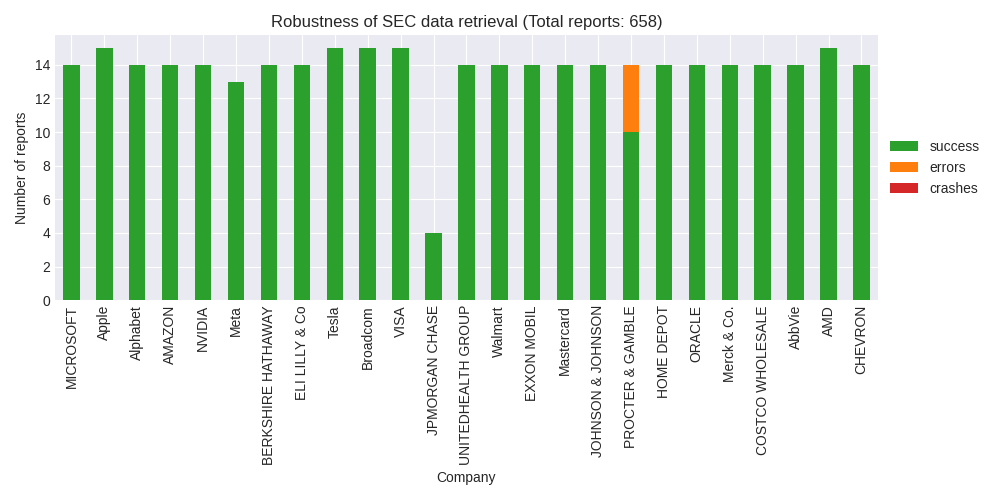
\includegraphics[width=1\textwidth]{images/robustness_1.png}
    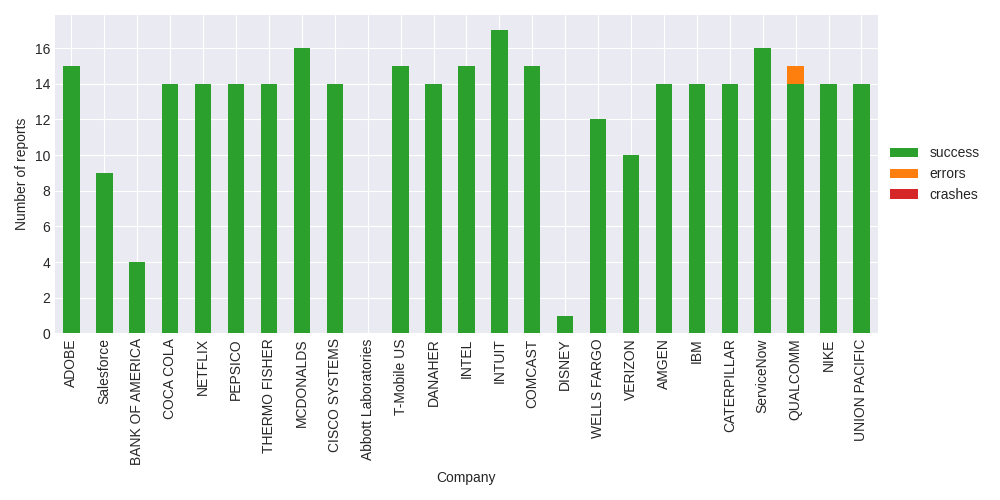
\includegraphics[width=1\textwidth]{images/robustness_2.png}
    \caption{Robustness evaluation of Brel}
    \label{fig:robustness}
\end{figure}

% The figure \ref{fig:robustness} shows the robustness evaluation of Brel.
% It shows the number of reports that were loaded successfully, with warnings or errors, 
% and the number of reports that caused Brel to crash.
% The figure shows that Brel was able to load 100\% of both 10K and 10Q reports without crashing.
% However, Brel logged warnings or errors for 0.76\% of the 10K and 10Q reports.
% These errors are caused by reports of the companies Procter \& Gamble and Qualcomm,
% which contain dimensions that reference concepts instead of explicit members.
% From a syntactic point of view, the XBRL specification allows for dimensions to reference concepts.
% However, from a logical point of view, using line items instead of dimensions is the correct way to model a dimension that references concepts.
% This is why Brel raises a warning for these reports.

% Note that this evaluation covers a different number of reports depending on the company.
% This was due to the fact that the SEC's API for fetching reports is not fully featured.
% One cannot specify the format of the report that one wants to fetch.
% Some of the reports returned by the API are in XML format, while others are in HTML format.
% Brel can only load reports in XML format.

% The robustness evaluation shows that Brel is robust against real-world XBRL reports.
% Even though Brel logged warnings or errors for 0.76\% of the reports, it was still able to load all of them.
% Once Brel supports opening hypercubes, it will be able to load 100\% of the reports without logging any warnings or errors.
% We can conclude that Brel is robust against real-world XBRL reports.
Figure \ref{fig:robustness} presents the robustness assessment of Brel, 
with individual companies represented on the x-axis.
% indicating the number of reports loaded successfully, those loaded with warnings or errors, 
% and instances where Brel encountered a failure on the y-axis.
% The individual companies are represented on the x-axis.
The y-axis displays the cumulative number of reports loaded successfully, with warnings or errors, and those that caused Brel to crash.
% , with the y-axis displaying their cumulative number success, warnings or errors, and failures.

Remarkably, Brel managed to process all 10K and 10Q reports without any failures across 658 reports.
Nonetheless, it encountered warnings or errors in 0.76\% of these reports, 
specifically from companies like Procter \& Gamble and Qualcomm. 
These issues arose from reports where dimensions referenced concepts rather than explicit members. 
While the XBRL specification technically permits dimensions to reference concepts, logically, 
% employing line items rather than dimensions is deemed more appropriate for modeling dimensions that refer to concepts.
a correct approach for modeling dimensions that reference concepts is to create a copy of the concept as a member. 
Therefore, this is a modeling error, and Brel issues warnings for such reports.
% Hence, Brel issues warnings for such reports.

The variation in the number of reports evaluated per company is attributed to limitations within the SEC's report retrieval API, 
which lacks the functionality to filter reports by format. 
Consequently, the API returns reports in either XML or HTML format, but Brel is only equipped to process XML-formatted reports.

% This robustness evaluation underscores Brel's capacity to handle real-world XBRL reports effectively. 
Despite logging warnings or errors for a small fraction of the reports, 
Brel's ability to load all reports demonstrates its robustness in processing real-world XBRL reports.
